\chapter{System Analysis}
The given setup being described, it is necessary to study its natural behavior in more details by deriving a model of this system. This chapter shows the process used to put up this model and an analyze of its pertinence. With this model, it shall possible, further on, to determine realistic requirements for the controllers to implement in this project, see \chapref{chap:requirements}.

As a start to this modelling, a mechanical drawing of the Cubli showing angles and coordinate system conventions is seen in \figref{cubliMechanical}.

\begin{figure}[H]
 \centering
 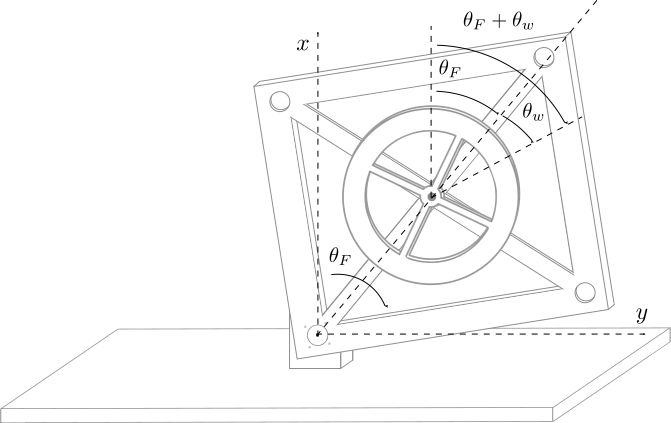
\includegraphics[scale=0.6]{figures/mechanicalSystem}
 \caption{Mechanical drawing of the Cubli, including angle coordinate system conventions}
 \label{cubliMechanical}
\end{figure}

In the next section, a complete model of the given setup is derived from Newton's Second Law of motion and rotation.